\documentclass{standalone}
\usepackage{pgfplots}
\usepackage{sansmath}
\pgfplotsset{compat=1.16}
\definecolor{ryu}{HTML}{3366FF}
\definecolor{std}{HTML}{949494}
\definecolor{bg}{HTML}{CFCFCF}
\begin{document}
\pagecolor{white}
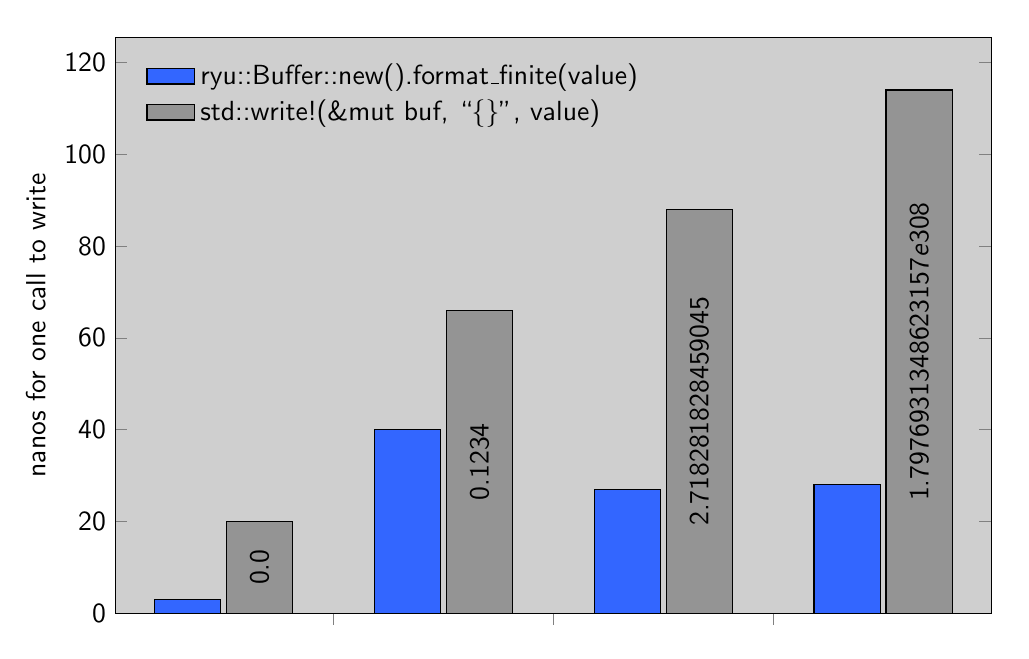
\begin{tikzpicture}
\edef\entries{
  "$0.0$",
  "$0.1234$",
  "$2.718281828459045$",
  "$1.7976931348623157e308$",
}
\begin{axis}[
  width=5in,
  height=3.5in,
  ybar,
  ymin=0,
  bar width=24pt,
  enlarge x limits={abs=39pt},
  ylabel={nanos for one call to write},
  legend style={
    anchor=north west,
    at={(0.025,0.975)},
    legend columns=1,
    draw=none,
    fill=none,
  },
  legend entries={
    ryu::Buffer::new().format\_finite(value)\\
    std::write!(\&mut buf, ``\{\}'', value)\\
  },
  legend cell align=left,
  xtick={-0.5,0.5,1.5,2.5,3.5,4.5},
  xticklabels={},
  xtick pos=left,
  visualization depends on={y \as \rawy},
  every node near coord/.append style={
    shift={(axis direction cs:0,-\rawy/2)},
    rotate=90,
    anchor=center,
    font=\sansmath\sffamily,
  },
  axis background/.style={fill=bg},
  tick label style={font=\sansmath\sffamily},
  every axis label={font=\sansmath\sffamily},
  legend style={font=\sansmath\sffamily},
  label style={font=\sansmath\sffamily},
]
  \addplot[
    black,
    fill=ryu,
    area legend,
    nodes near coords={},
  ] coordinates {
    (0, 3)
    (1, 40)
    (2, 27)
    (3, 28)
  };
  \addplot[
    black,
    fill=std,
    area legend,
    nodes near coords=\pgfmathsetmacro{\input}{{\entries}[\coordindex]}\input,
  ] coordinates {
    (0, 20)
    (1, 66)
    (2, 88)
    (3, 114)
  };
\end{axis}
\pgfresetboundingbox\path
  (current axis.south west) -- ++(-0.44in,-0.09in)
  rectangle (current axis.north east) -- ++(0.05in,0.05in);
\end{tikzpicture}
\end{document}
